\documentclass[a4paper, 14pt]{article}
\usepackage{float}
\usepackage{geometry}
\usepackage{graphicx}
\usepackage[utf8]{inputenc}
\usepackage{setspace}
\usepackage{lmodern}
\usepackage[hidelinks]{hyperref}

\linespread{1.5}
\newcommand\tab[1][1cm]{\hspace*{#1}}
\geometry{left=20mm,right=20mm,top=20mm,bottom=20mm}
\begin{document}
\fontfamily{ptm}\selectfont
{
\pagenumbering{arabic}
\begin{center}	
\textbf{\fontsize{18}{2} \selectfont POST MERGER ANALYSIS OF CUSTOMER SATISFACTION AND LOYALTY - A STUDY ON RECENT MERGER OF ASSOCIATE BANKS OF SBI WITH ITSELF}\\
\tab \\
\textbf{\fontsize{14}{2} \selectfont REVIEW 3 - REPORT}\\
\tab \\
\textbf{\fontsize{14}{2} \selectfont \emph{Submitted by}}\\
\tab \\
\tab \\
{\fontsize{16}{2} \selectfont
\textbf{ADHITHYAN V}}\\
{\fontsize{16}{2} \selectfont \textbf{(2016201002)}}\\

\textbf{\fontsize{16}{2} \selectfont MASTER OF BUSINESS ADMINISTRATION}\\
\begin{figure}[H]
\centering

\includegraphics[scale=0.5]{anna_univ_logo.jpg}
\end{figure}
\tab \\
\textbf{\fontsize{14}{2} \selectfont COLLEGE OF ENGINEERING, GUINDY}\\
\tab \\
\textbf{\fontsize{16}{2} \selectfont ANNA UNIVERSITY : CHENNAI 600 025}\\
\tab \\
{\fontsize{14}{2} \selectfont APRIL 2018}\\
\end{center}
\newpage
\section*{DATA COLLECTION}
\par Data was collected in 2 modes \textbf{online} mode using \textbf{Google Forms} and \textbf{offline mode} in which some part of data was collected from erstwhile SBT pollachi branch and SBH Thiruvanmiyur branch. For online mode data collection twitter was used as medium to communicate with people. Those who have mentioned SBH, SBT, SBBJ, SBP and SBM were identified from their tweets and they were contacted to obtain response.
\section*{ANALYSIS}
\subsection*{No of data}
\par A total of \textbf{101} responses were obtained using Google forms and some of the data was collected in the bank premises in Chennai and Pollachi.
\subsection*{Demographics}
\par Out of 101 responses
\begin{itemize}
\item 17 were Female (16.8 \%)
\item 84 were Male (83.2 \%)
\end{itemize}
\begin{figure}[H]
\centering
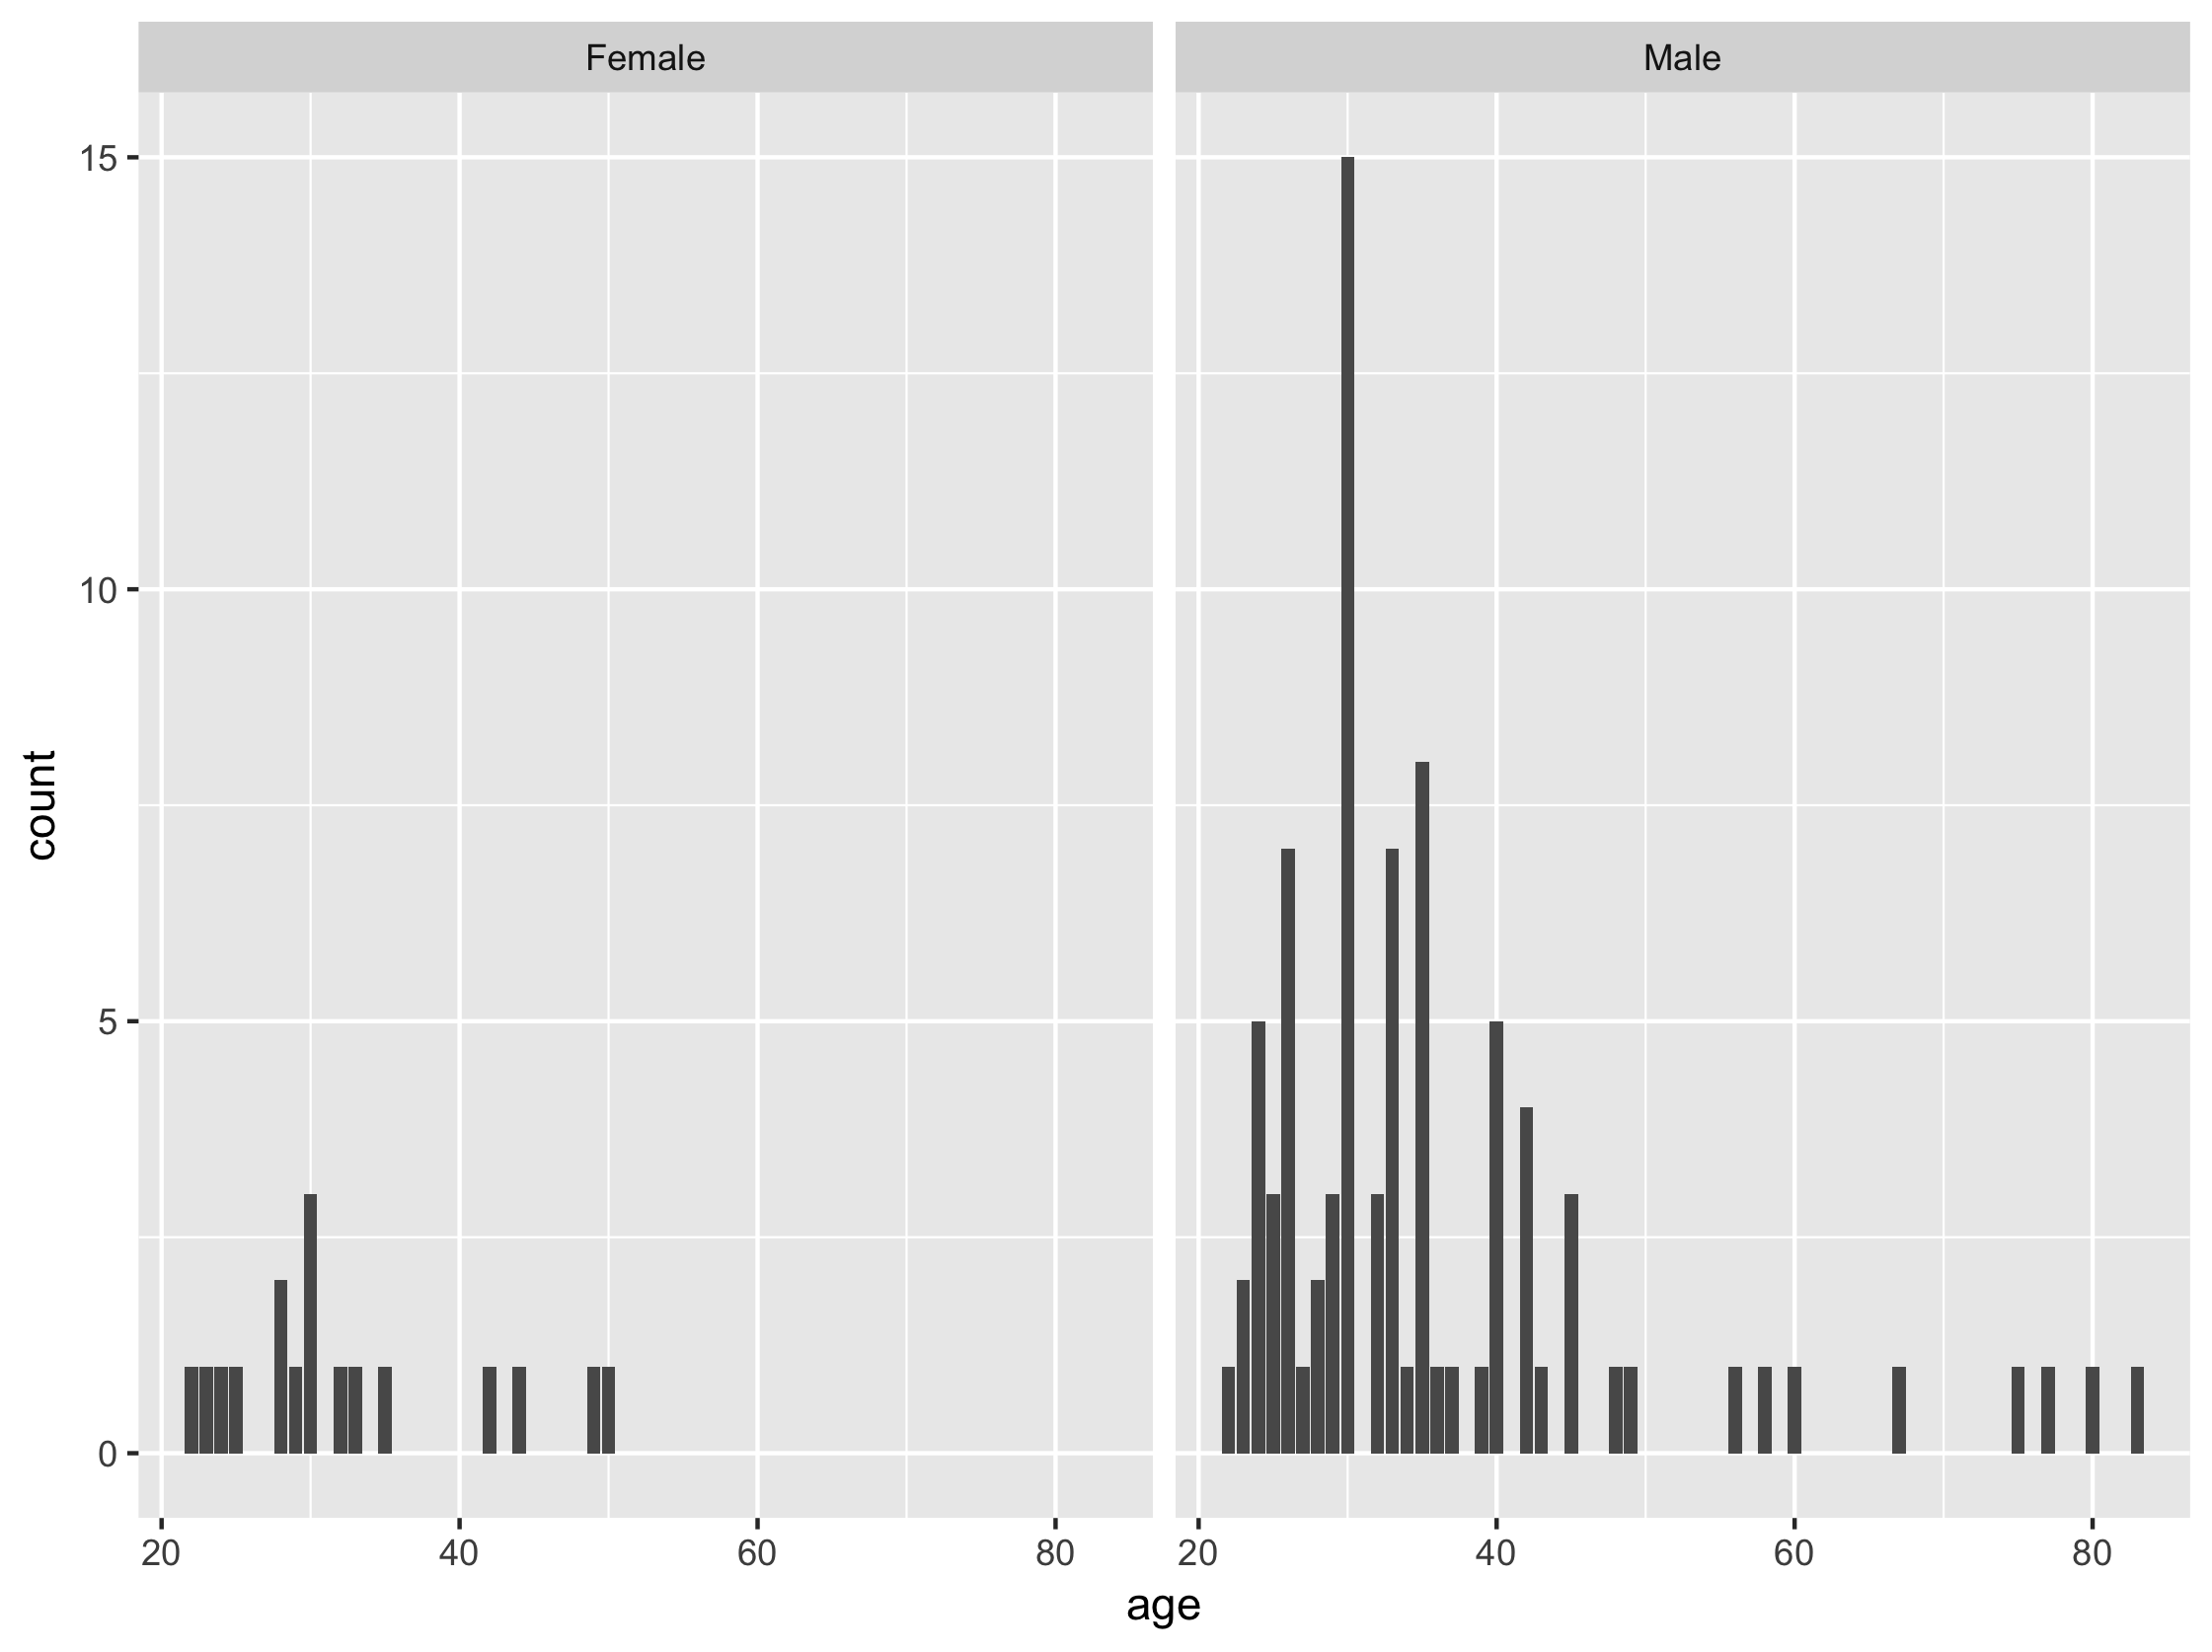
\includegraphics[scale=0.2]{age_distribution.png}
\caption{Age distribution of respondents}
\end{figure}
\subsection*{Cronbach's alpha}
\begin{center}
\begin{tabular}{|c|c|c|}
\hline
\textbf{Scale name} & \textbf{Cronbach $\alpha$} & \textbf{No of items}\\
\hline
Psychological Contract Violation & \textbf{0.218} & 8\\
Service Performance & \textbf{0.712} & 10\\
Customer Satisfaction & \textbf{0.96} & 4\\
Customer Loyalty & \textbf{0.927} & 5 \\
\hline
\end{tabular}
\end{center}

\subsection*{DESCRPTIVE STATISTICS}
\begin{center}
\begin{tabular}{|c|c|c|c|}
\hline
Item & \textbf{Mean} & \textbf{SD} & N \\
\hline
Customer satisfaction & 2.7847 & 1.33706 & 101 \\
PCV & 2.87005 & .503091 & 101 \\
Overall service & 2.8 & 1.49 & 101 \\
Service performance & 2.81 & .6437 & 101 \\
Loyalty & 2.685 & .368 & 101 \\
\hline
\end{tabular}
\end{center}

\subsection*{HYPOTHESIS}
\begin{itemize}
\item H1 - Psychological Contract Violation has negative influence on customer satisfaction.
\item H2 - Service performance is a determinant of Overall Service
\item H3 - Overall service has a positive impact on customer satisfaction
\item H4 - Customer satisfaction has positive influence on customer loyalty.
\end{itemize}

\subsection*{Pearson Correlation}
\begin{center}
\begin{tabular}{|c|c|}
\hline
Variables & Correlation Value \\
\hline
PCV vs Customer Satisfaction & \textbf{-0.638} \\
Service Performance vs Overall Service & \textbf{-0.744} \\
Overall service vs Customer Satisfaction & \textbf{0.949} \\
Customer Satisfaction vs Customer Loyalty & \textbf{0.396} \\
\hline
\end{tabular}
\end{center}

\subsection*{MODEL SUMMARY}
\begin{figure}[H]
\centering
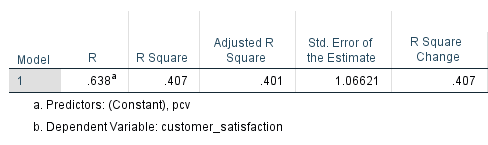
\includegraphics[scale=1]{pcv_vs_customer_satisfaction.png}
\end{figure}

\begin{figure}[H]
\centering
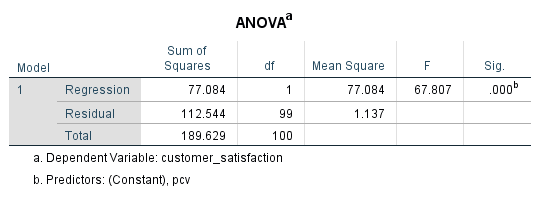
\includegraphics[scale=1]{anova_pcv_cs.png}
\caption{H1 - Psychological Contract Violation has negative influence on customer satisfaction.}
\end{figure}


\begin{figure}[H]
\centering
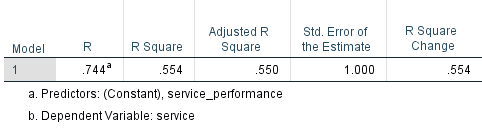
\includegraphics[scale=1]{service_performance_vs_service.png}
\end{figure}

\begin{figure}[H]
\centering
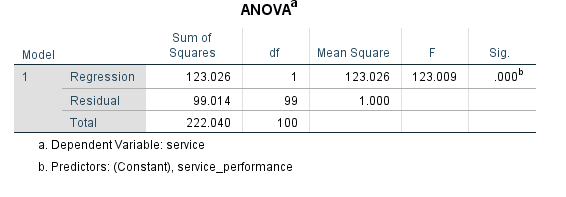
\includegraphics[scale=1]{anova_s_sp.png}
\caption{H2 - Service performance is a determinant of Overall Service}
\end{figure}


\begin{figure}[H]
\centering
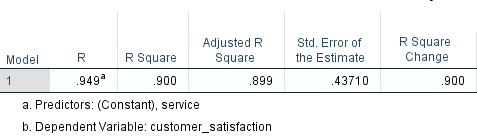
\includegraphics[scale=1]{sp_vs_cs.png}
\end{figure}

\begin{figure}[H]
\centering
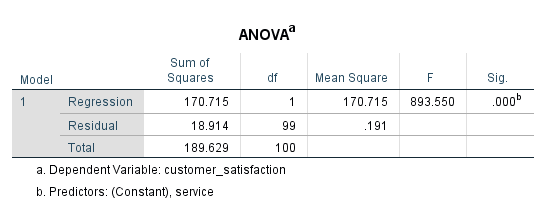
\includegraphics[scale=1]{anova_css.png}
\caption{H3 - Overall service has a positive impact on customer satisfaction}
\end{figure}

\begin{figure}[H]
\centering
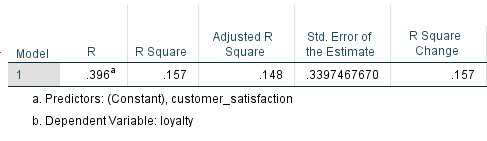
\includegraphics[scale=1]{customer_satisfaction_vs_loyalty.png}
\end{figure}

\begin{figure}[H]
\centering
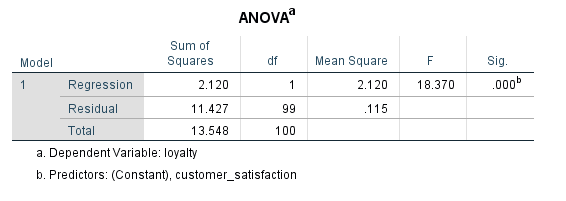
\includegraphics[scale=1]{anova_cs_lo.png}
\caption{H4 - Customer satisfaction has positive influence on customer loyalty.}
\end{figure}

\section*{INTERPRETATION}
\begin{itemize}
\item PCV and customer satisfaction are negatively correlated (-0.638). This indicates as customer perceives more PCV, satisfaction declines. \textbf{H1 is accepted}
\item Service performance is negatively correlated with overall service (-0.744). This indicates overall service doesn't depend on service performance. \textbf{H2 is rejected}
\item Overall service has a positive correlation with customer satisfaction (0.949). As overall service increases, customer satisfaction tends to increase. 
\textbf{H3 is accepted}
\item Customer satisfaction and loyalty are postively correlated (0.349). This indicates a satisfied customer will be more loyal to the bank and spreads word of mouth.\textbf{H4 is accepted.}
\item PCV explains 40.1\% variance in customer satisfaction.
\item Service performance explains 55\% of variance in overall service.
\item Overall service explains 89.9\% of variance in customer satisfaction.
\item Customer satisfaction explains 15.7\% of variance in loyalty.
\end{itemize}
\section*{CONCLUSION}
\par Though merger is beneficial to management in terms of financial perspective and synergies, merger often brings a lot of pain to customer. In our case many branches were shut down, customers lost identities etc. So merger should be planned with customer in mind to ensure smooth functioning and service.
\section*{FUTURE RESEARCH DIRECTIONS}
\par During response collection it was found that, many of the people preferred private banks over SBI/PSU banks. So a study can be conducted to know the areas in which private banks excel and it can be used to improve the service of PSU banks.
}
\end{document}